\documentclass[aspectratio=169,11pt]{beamer}
\usetheme{Madrid}
\usecolortheme{default}
\usepackage{xeCJK}
\setCJKmainfont{Hiragino Sans}
\setCJKsansfont[BoldFont=Hiragino Kaku Gothic W8]{Hiragino Kaku Gothic W6}
\setCJKmonofont{Hiragino Sans Mono}
\usepackage{fontspec}
\usepackage{graphicx}
\usepackage{booktabs}
\usepackage{amsmath}
\usepackage{hyperref}
\setbeamertemplate{navigation symbols}{}
\setbeamertemplate{footline}[frame number]
\title{実データと生成データの識別に向けた時系列分析}
\subtitle{Stylized Facts と生成モデルの検討}
\author{DSS mizuho group3}
\date{\today}

\begin{document}

\begin{frame}
  \titlepage
\end{frame}

\begin{frame}{目的と方針}
\begin{block}{目的}
S\&P500 と DGS10 の時系列について，実データと生成データを識別できる特徴量を探す。
\end{block}
\begin{itemize}
  \item 価格水準・リターン分布・ボラティリティ系列を比較する。
  \item GBM や SABR などの生成モデルが再現できる性質／苦手な性質を整理する。
  \item 識別に使えそうな stylized facts を抽出し，生成側の改良方針につなげる。
\end{itemize}
\end{frame}

\begin{frame}{GBM: 観察された特徴}
\begin{columns}[T]
\begin{column}{0.55\textwidth}
\begin{itemize}
  \item GBM はあくまでドリフト項 + 正規分布
    \item ファットテールを再現しにくい
    \item リターン分布の非対称性も再現しにくい
  \item 歪度・尖度を見ると，mask2 と mask4 が特徴的
  \item 相関係数では mask2, mask3 が多く検出された
\end{itemize}
\end{column}
\begin{column}{0.42\textwidth}
\centering
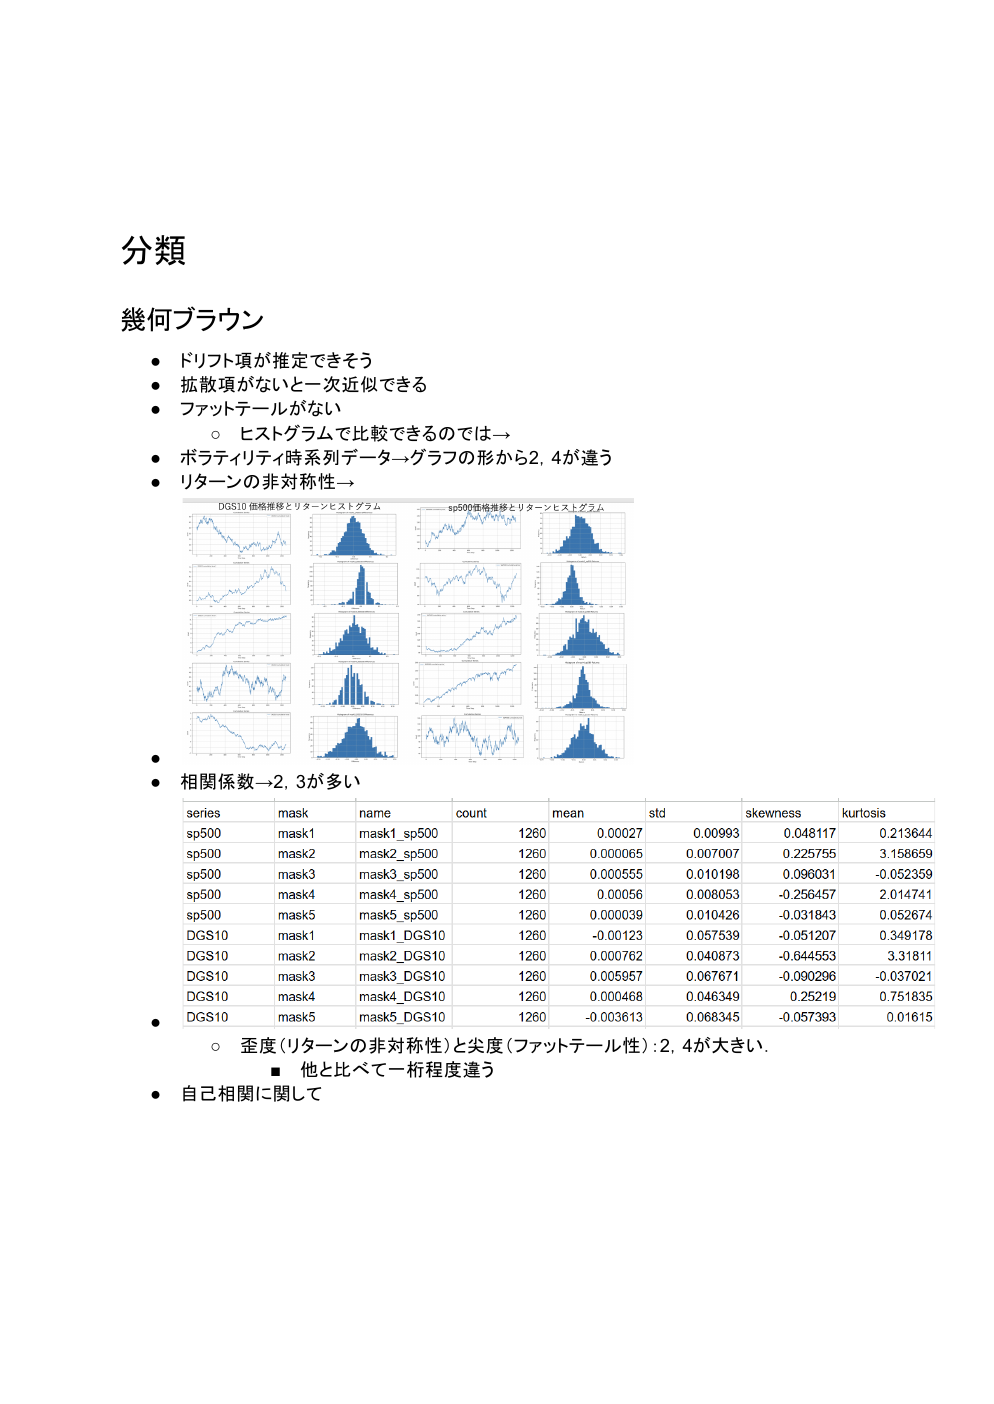
\includegraphics[height=0.62\textheight,keepaspectratio]{rendered/page-1.png}
\end{column}
\end{columns}
\end{frame}

\begin{frame}{GBM: 自己相関とレバレッジ効果}
\begin{columns}[T]
\begin{column}{0.52\textwidth}
\begin{itemize}
  \item リターンの自己相関は，lag によって評価が変わる。
  \item rolling volatility と return の相関を用いて，レバレッジ効果を確認した。
  \item GBM だけでは，下落時にボラティリティが上がる性質を十分に表しにくい。
\end{itemize}
\end{column}
\begin{column}{0.45\textwidth}
\centering
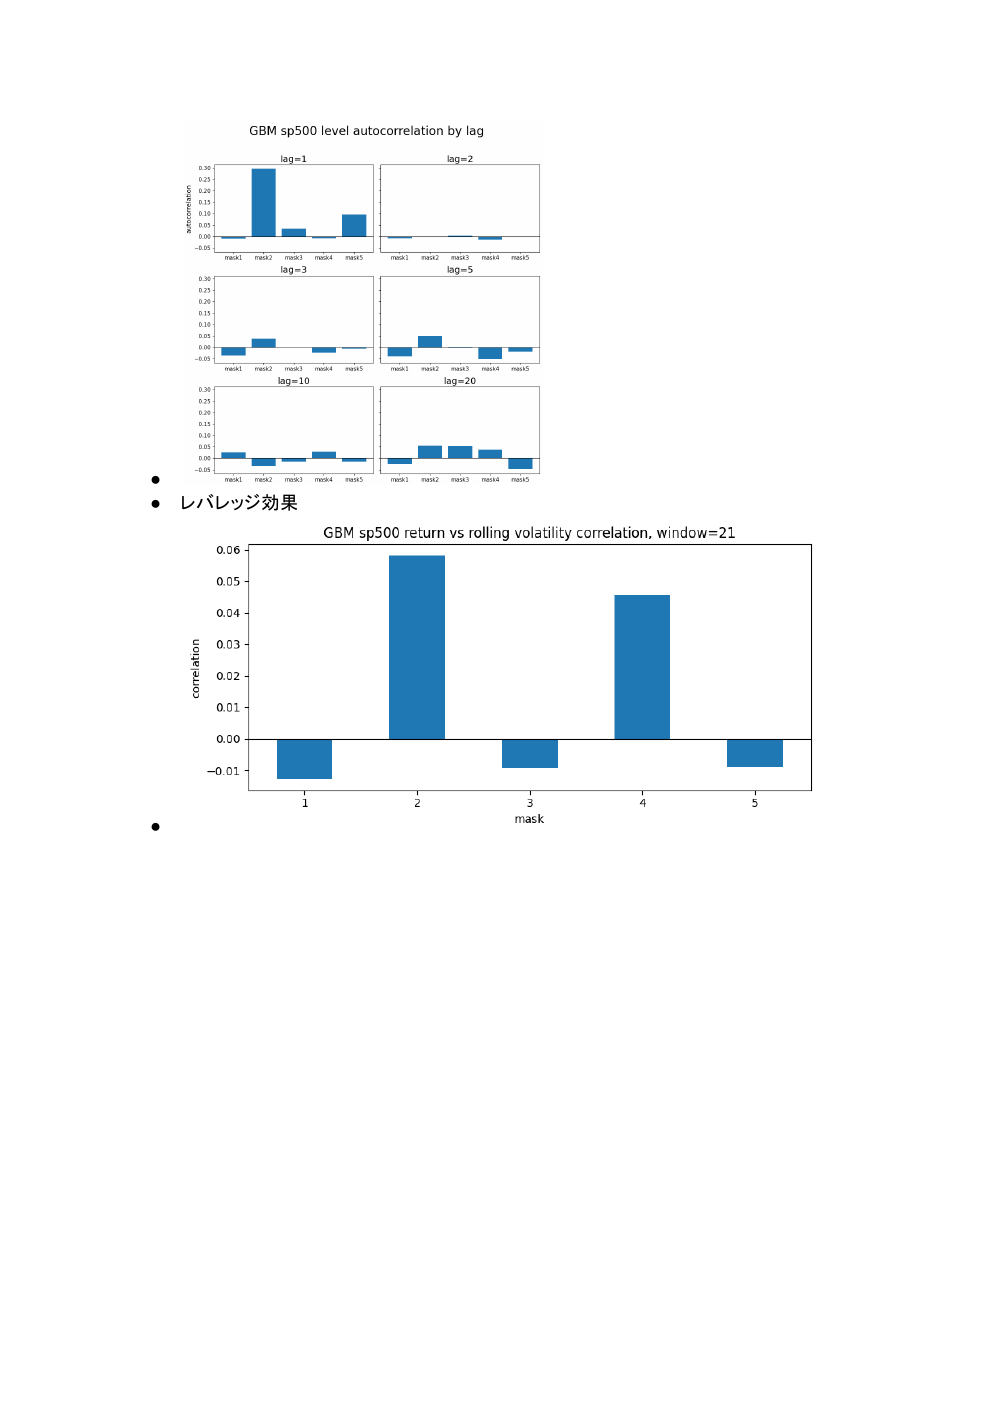
\includegraphics[height=0.62\textheight,keepaspectratio]{rendered/page-2.png}
\end{column}
\end{columns}
\end{frame}

\begin{frame}{SABRモデル: 再現できる性質}
\begin{columns}[T]
\begin{column}{0.55\textwidth}
\begin{itemize}
  \item SABR はボラティリティ自体を確率過程として扱う。
  \item そのため，ボラティリティクラスタリングを表現しやすい。
  \item リターン分布の非対称性では mask2 と mask5 が特徴的。
  \item ただし，ファットテールやクラスタリングだけでは識別根拠として弱い。
\end{itemize}
\end{column}
\begin{column}{0.42\textwidth}
\centering
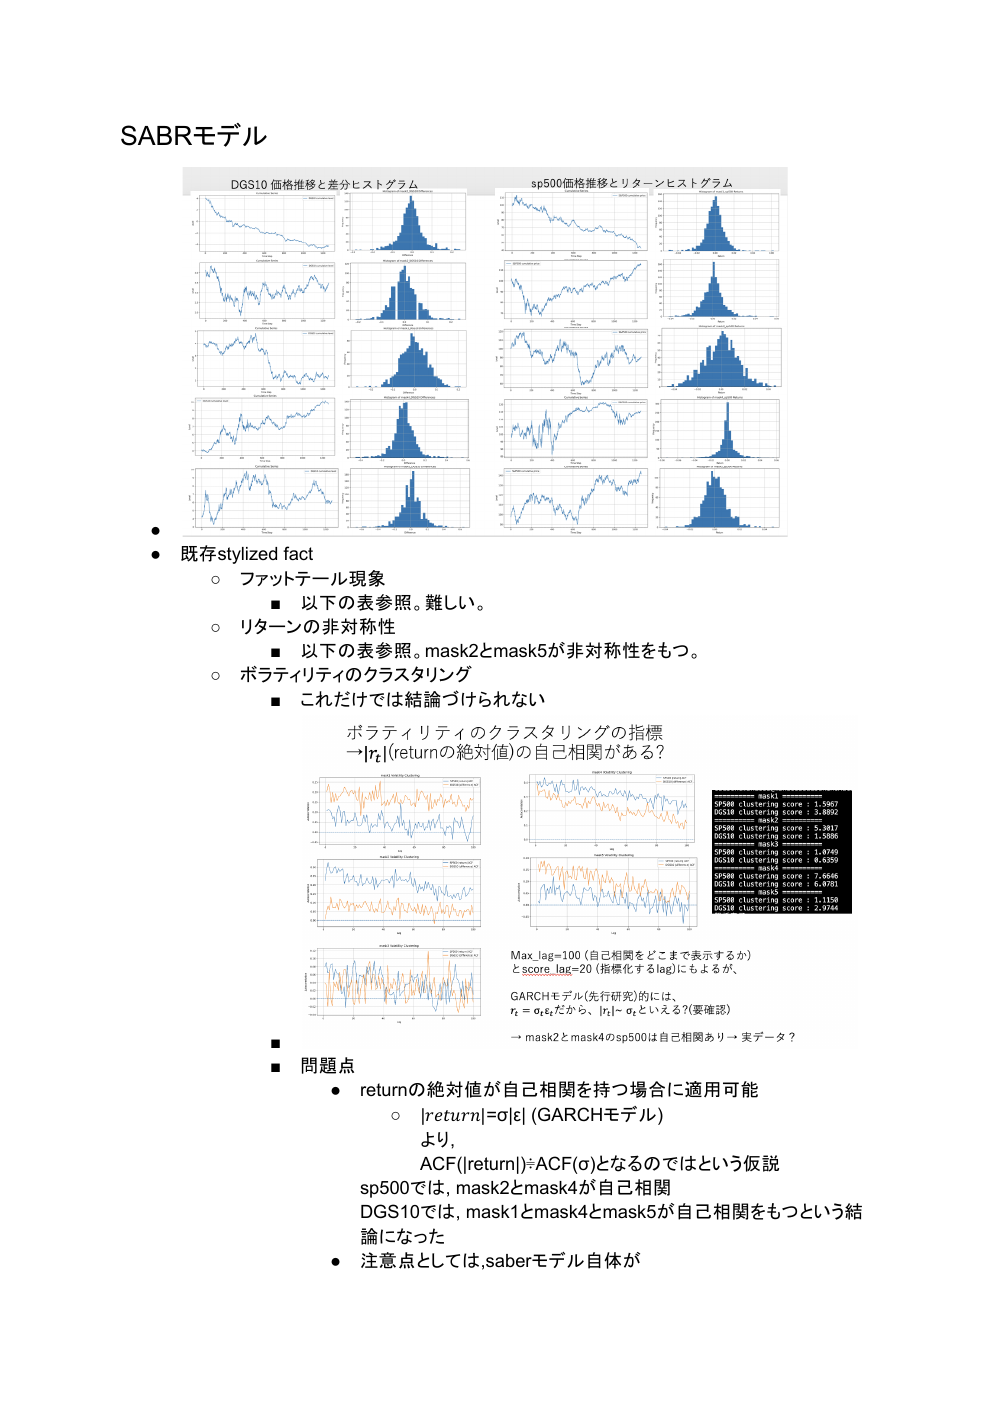
\includegraphics[height=0.62\textheight,keepaspectratio]{rendered/page-3.png}
\end{column}
\end{columns}
\end{frame}

\begin{frame}{SABRモデル: 識別の難しさ}
\begin{block}{ポイント}
\[
  d\sigma_t = \nu\sigma_t\,dW_t
\]
SABR ではボラティリティが確率過程に組み込まれているため，生成データでも強い自己相関が出る可能性がある。
\end{block}
\begin{itemize}
  \item 実データでも SABR でも，$|\mathrm{return}|$ は自己相関を持ちうる。
  \item したがって，ボラティリティクラスタリング単独では識別が難しい。
  \item 追加で，レバレッジ効果・相関の時間変化・相関の非対称性を見る必要がある。
\end{itemize}
\end{frame}

\begin{frame}{追加で見たい特徴量}
\begin{columns}[T]
\begin{column}{0.48\textwidth}
\textbf{単一時系列の特徴}
\begin{itemize}
  \item ファットテール
  \item リターン分布の非対称性
  \item ボラティリティクラスタリング
  \item リターンの自己相関の弱さ
  \item レバレッジ効果
\end{itemize}
\end{column}
\begin{column}{0.48\textwidth}
\textbf{複数時系列間の特徴}
\begin{itemize}
  \item 相関の時間依存性
  \item 相関の非対称性
  \item 高ボラティリティ局面での相関増加
  \item 株価下落時の DGS10 との関係
  \item リード・ラグ現象
\end{itemize}
\end{column}
\end{columns}
\end{frame}

\begin{frame}{試した識別手法と限界}
\begin{columns}[T]
\begin{column}{0.53\textwidth}
\begin{itemize}
  \item 順列エントロピーにより volatility complexity を比較。
  \item 結果から mask2, mask5 が怪しい候補として得られた。
  \item Markov Switching Model で尤度比較も行った。
  \item ただし，単純なモデルでは生成データにも良い尤度が出てしまい，決定打にはならなかった。
\end{itemize}
\end{column}
\begin{column}{0.44\textwidth}
\centering
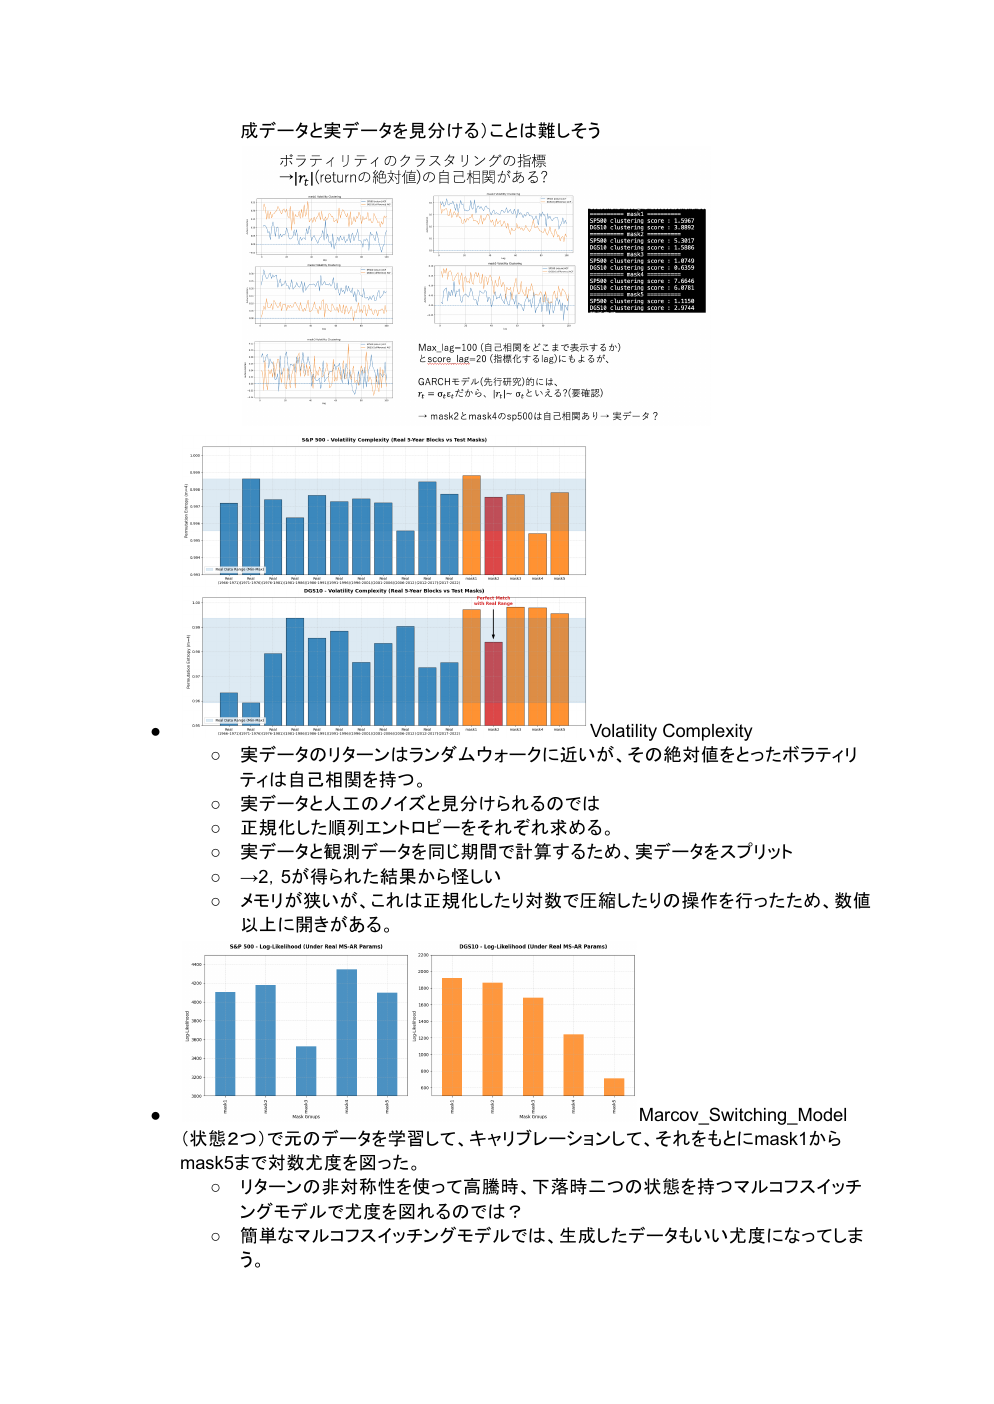
\includegraphics[height=0.62\textheight,keepaspectratio]{rendered/page-6.png}
\end{column}
\end{columns}
\end{frame}

\begin{frame}{生成側の目標}
\begin{block}{目標}
Stylized facts による識別が通用しにくい時系列を生成する。
\end{block}
\begin{itemize}
  \item まずは既存の金融時系列の stylized facts をできるだけ再現する。
  \item 単一時系列では，ファットテール・非対称性・クラスタリング・レバレッジ効果を再現する。
  \item 複数時系列では，相関の時間変化・下落時の相関変化・高ボラ局面の依存構造を再現する。
\end{itemize}
\end{frame}

\begin{frame}{候補となる生成モデル}
\begin{columns}[T]
\begin{column}{0.5\textwidth}
\textbf{比較的シンプルなモデル}
\begin{itemize}
  \item 区間 Bootstrap
  \item GARCH
  \item GJR-GARCH
  \item ADCC-GARCH
  \item Markov Switching Model
\end{itemize}
\end{column}
\begin{column}{0.5\textwidth}
\textbf{複雑なモデル}
\begin{itemize}
  \item Jump diffusion
  \item Rough volatility
  \item Copula + GARCH
  \item Stochastic volatility
  \item Quant GAN / Signature Wasserstein GAN
  \item Diffusion / CSDI / SigDiffusion
\end{itemize}
\end{column}
\end{columns}
\end{frame}

\begin{frame}{まとめ}
\begin{itemize}
  \item GBM は単純だが，ファットテールやレバレッジ効果の再現が弱い。
  \item SABR はボラティリティ過程を持つため，クラスタリングは再現しやすい。
  \item 一方で，クラスタリングだけでは実データ／生成データの識別は難しい。
  \item 今後は，単一時系列の stylized facts と複数時系列間の依存構造を同時に見る。
\end{itemize}
\begin{block}{次の一手}
GARCH 系・Copula・Regime Switching をベースラインにし，深層生成モデルと比較する。
\end{block}
\end{frame}

\end{document}
